\section{Executive information systems}

Executive information systems are designed to provide senior leaders with the tools and insights they need to make informed, strategic decisions. 
These systems integrate data from various functional areas of an organization into a cohesive framework: 
\begin{itemize}
    \item \textit{Financial performance}: monitor and optimize the financial health of the organization.
        Planning, budgeting and reporting with Activity Based Costing. 
    \item \textit{Process performance}: evaluate and enhance the efficiency of internal processes.
        Management dashboards  with input-output process models
    \item \textit{Clients and markets}: understand and engage with customers and markets effectively.
        Executive CRM with analytical CRM 
    \item \textit{Innovation and critical resources}: foster innovation and manage critical resources strategically.
        Strategic planning with strategic control (balanced scorecard). 
    \item \textit{Information to stakeholders}: communicate effectively with internal and external stakeholders.
        Communication through portals.
\end{itemize}

\begin{figure}[H]
    \centering
    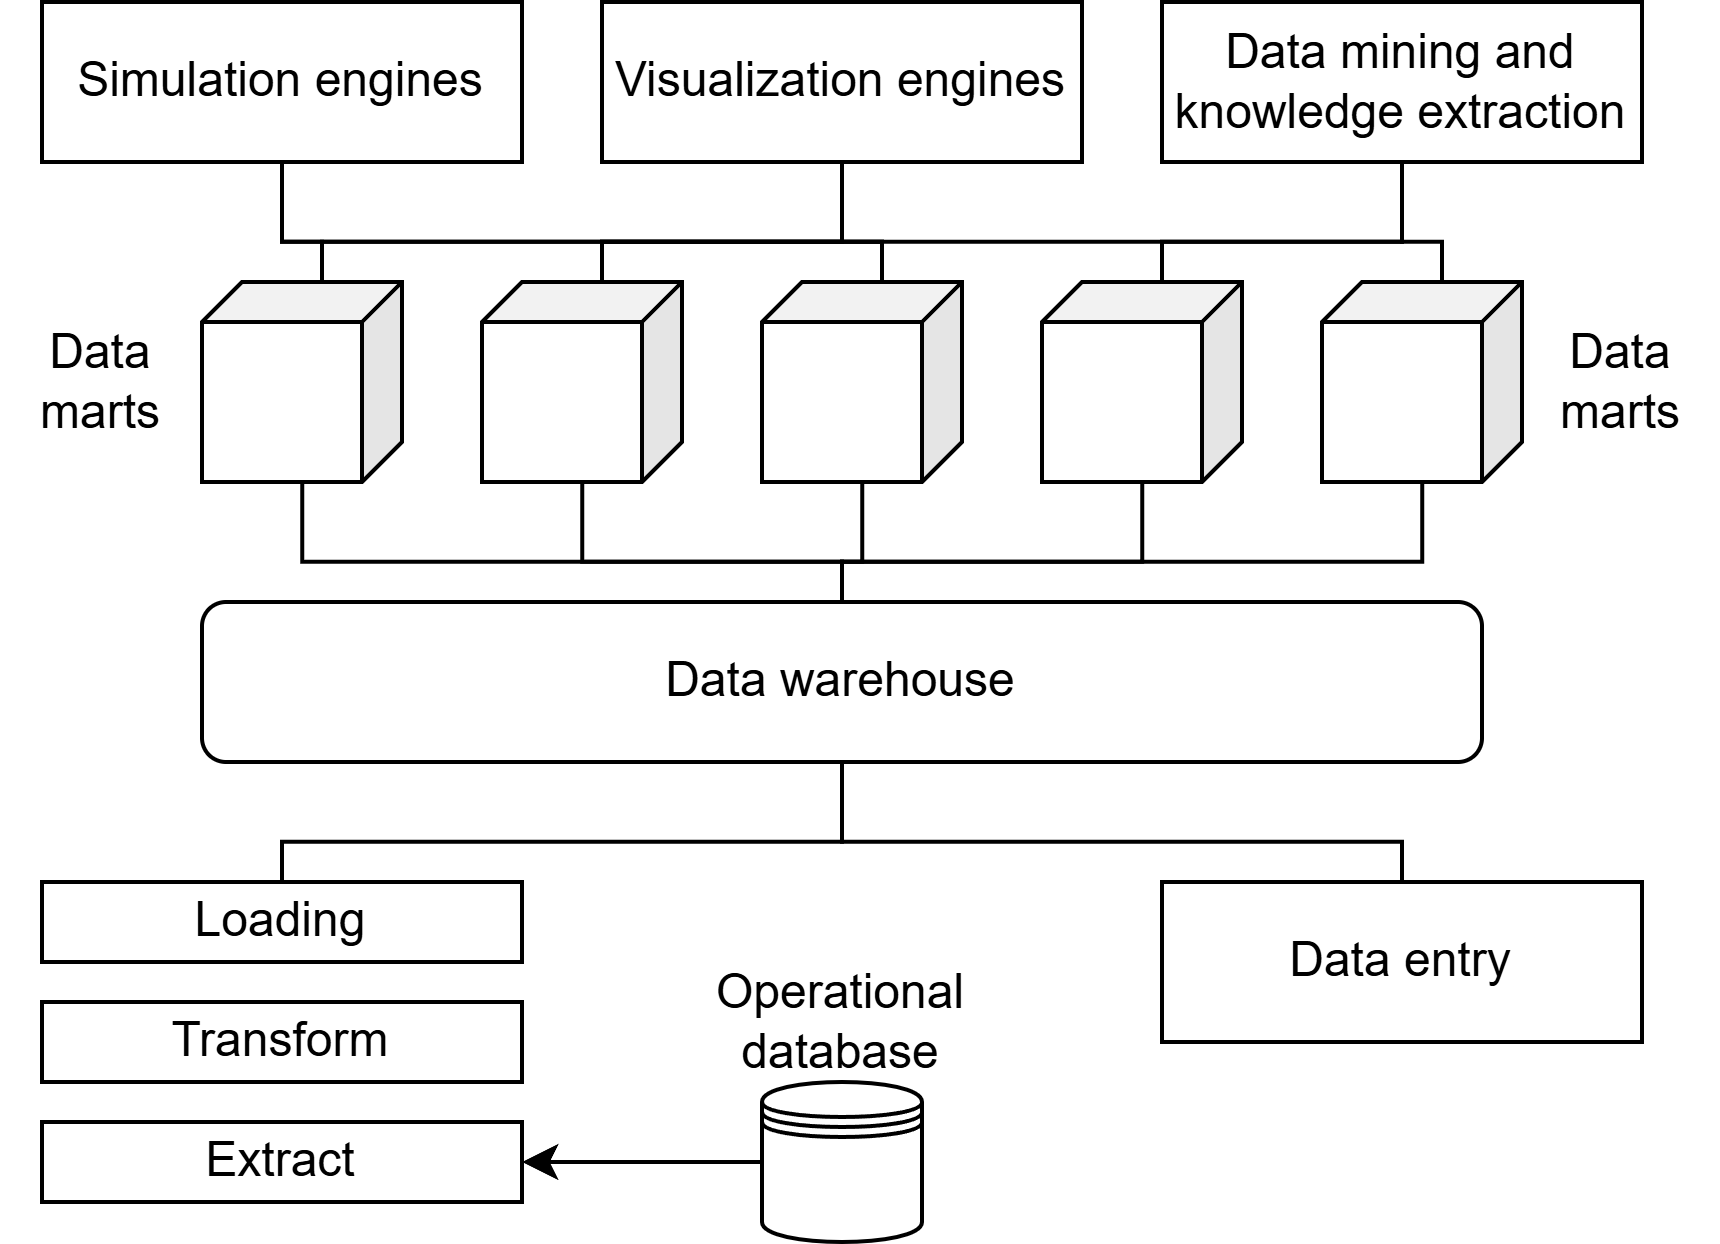
\includegraphics[width=0.5\linewidth]{images/bis4.png}
    \caption{Executive information system}
\end{figure}
At the heart of an executive information systems are Key Performance Indicators (KPI): metrics that summarize the performance of specific activities or parameters. 
These indicators are defined by multiple dimensions, including: time, organizational unit, customer, product, process and activity, and other dimensions.